\documentclass{article}

% if you need to pass options to natbib, use, e.g.:
%     \PassOptionsToPackage{numbers, compress}{natbib}
% before loading tex file

% to compile a preprint version, e.g., for submission to arXiv, add the
% [preprint] option:
%  \usepackage[preprint]{neurips_2020}

% to compile a camera-ready version, add the [final] option, e.g.:
%     \usepackage[final]{neurips_2020}

% to avoid loading the natbib package, add option nonatbib:
%    \usepackage[preprint, nonatbib]{neurips_2020}

\usepackage{arxiv}
\usepackage[utf8]{inputenc} % allow utf-8 input
\usepackage[T1]{fontenc}    % use 8-bit T1 fonts
\usepackage{hyperref}       % hyperlinks
\usepackage{url}            % simple URL typesetting
\usepackage{booktabs}       % professional-quality tables
\usepackage{amsfonts}       % blackboard math symbols
\usepackage{nicefrac}       % compact symbols for 1/2, etc.
\usepackage{microtype}      % microtypography
\usepackage{graphicx}
\usepackage{caption}
\usepackage{subcaption}

\graphicspath{ {./images/} }

\pagestyle{fancy} 
\lhead{IRAP Poject Code: \texttt{Q2019-1697}}
\chead{KOHO Financial}
\rhead{01/12/2020 - 06/30/2020}

\fancypagestyle{disclaimer-footer}{%
  \fancyhf{}
  \renewcommand\headrulewidth{0pt}
  \fancyfoot[C]{\tiny Strictly confidential report. Do not reproduce or use in any way, without the prior written consent of the Company 
(except for archiving, \underline{provision of consulting services and assessment} purposes by the concerned Parties).}
}

\title{Representational Models of Consumer Spending}

\author{%
  Josh Harris \thanks{IRAP Poject Code: \texttt{Q2019-1697}}\\
  KOHO Financial\\
  Toronto, ON \\
  \texttt{josh@koho.ca} \\
  
  \And
  Ars\`{e}ne Fansi Tchango \\
  MILA \\
  Montreal, QC \\
  \texttt{arsene.fansi.tchango@mila.quebec}
}

\begin{document}

\maketitle

\thispagestyle{disclaimer-footer}

\begin{abstract}
  We frame consumer spending as users making sequences of transactions with various merchants. We train a neural net to make predictions about future transactions in the sequence, and examine the representational embeddings learned during training. We adopt state of the art methods developed for machine translation, and evaluate how well such methods apply to the consumer spending domain.
\end{abstract}

\section{Introduction}
KOHO Financial provides a payment card that is used to make purchases at a wide variety of merchants. KOHO seeks to deliver as much value to the user as it can afford, as an active participant in their financial wellbeing. One way it does this through cashback programs that may be more valuable to users when rewards are personalized. Other ways include services such as budgeting and financial planning which benefit from a positive relationship with users and a strong understanding of them.

\subsection{Motivation}
The choices a person makes about where to use their KOHO card say a lot about the role of KOHO in their life, and given enough usage, their financial needs and nuances. Currently this understanding of users is gained using explicit measurements and manual feature engineering based on common sense and industry wisdom. These tools are effective at capturing patterns and trends in easily measurable quantities, but lack insight into the development of more complex phenomena that are hard to measure directly. This work presents an additional method to enhance business insight into such phenomena, that can be optimized and naturally operates at population-scale.

The work described here aims to identify patterns in behavioural data by unlocking information contained in consumer spending behaviour, to reason about such behaviour in more detail. For this purpose we construct a model designed to learn numeric representations of users, and the merchants they frequent. It learns these while learning to predict which merchants users will choose for their upcoming transactions. The numeric representations are what we are really interested in, while the next merchant prediction as a means to produce them has it's own beneficial uses. The learned representations in an ideal case can potentially be used for knowledge discovery regarding relationships between merchants, between users and merchants, and between users and KOHO. 

\section{Hypothesis}
Our motivation rests on the hypothesis that representations learned by a properly constructed and trained neural network can capture some of the underlying structure found in consumer behaviour. The learned structure in these embedded representations should not only enable next merchant prediction, but also be useful in other in other applications. In essence it's an application of the generally accepted manifold hypothesis \cite{Fefferman:2013}, which gives a geometric explanation of why neural networks have proven so effective. In this work we explore this idea by extracting re-using representations as inputs to a different prediction by a different type of model, focusing on a subset of merchants as discussed below.

\section{Applications}
Our model is designed to produce two main levels of representation that both offer opportunities for solving KOHO’s business problems. Merchant representations can be used to develop more granular categories to enable more context-aware budgeting, and can help offer users the most useful power-ups. User representations can provide an understanding of how a user is adopting the product, and once they’ve adopted fully, how their lives are changing.

\section{Baseline Representations}
To produce a baseline for merchant representations we used the \texttt{gensim} python package, which implements an efficient algorithm for producing word representations \cite{Mikolov:2013}. We train it on sequences of merchants to produce an embedding for each merchant. This method is chosen because we know that \texttt{gensim} is able to embed semantic information into a representational space when applied to natural language, and we investigate if the same is true in the consumer spending domain. To obtain a representation of a user \textit{u} in this baseline scenario, we use: 

\begin{equation}
  u=\frac{\sum_{i=1}^S m_i}{S}
\end{equation}

which is the mean of merchant embeddings \textit{m} over a sequence of transactions of length \textit{S}. Using this as a baseline method sets the bar high for our learned representations. 

\begin{figure}
  \centering
  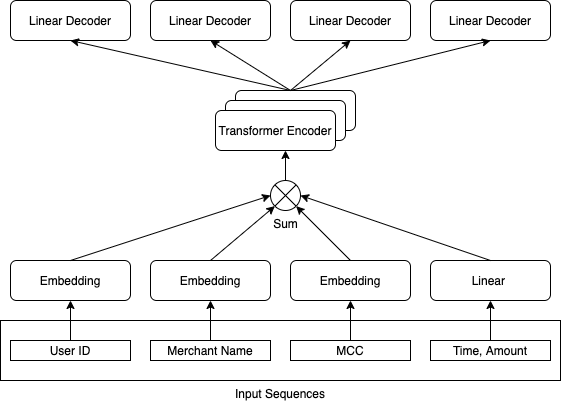
\includegraphics[width=.6\linewidth]{tx_sig.png}
  \caption{Outline of the model architecture used for next merchant prediction. Representations are taken from the embedding layers.}
  \label{arch}
\end{figure}

\section{Model Architecture}
The core model developed in this work learns its representations by taking ordered sequences of a user’s transactions to predict the next merchant name and other attributes of the next transaction for that user. The architecture depicted in Figure \ref{arch} is made up of embedding layers, Transformer \cite{Vaswani:2017} encoder layers, and linear decoder layers. The Transformer layers output a prediction for each position in the sequence. 

Training experiments were done using various features of transactions, keeping merchant name as the core feature in all experiments. The set of all merchant names is tokenized to form a vocabulary, and each transaction is a “word” choice from that vocabulary. Tokenized merchants are given to a trainable embedding layer. The ID of the user is also tokenized and given to another trainable embedding layer. Other features experimented with are; the time of day, day of week, and amount of the transaction, as well as the MCC (merchant category code) as configured by the merchant at each point of sale terminal. These inputs are combined and fed into some number of Transformer layers. On top of the transformer layers is a decoder for each feature other than user ID. Each decoder contributes to the total loss with a given weight. All features except amount are categorical and thus their decoders use a categorical cross entropy loss function. Amount is a continuous dollar value and so uses a mean squared error loss. An Adam optimizer with default settings is used to calculate parameter updates. Merchant and user representations are taken from their respective embedding layers.

\section{Evaluation Metrics}
These measures were used to evaluate the performance of the Transformer model.

\subsection{Recall@K}
During training, \textit{Recall@k} is used to select the best training runs, which measures the proportion of inputs where the target merchant is in the model’s top \textit{k} predictions. We use $k=1,3,10$ to calculate the number of elements in the intersection between the top \textit{k} predictions $\hat{y}$ and the ground truth labels \textit{y}

\begin{equation}
  Recall@k=\frac{n(\top_k\hat{y} \cap y)}{NS}
\end{equation}

over a training batch of \textit{N} sequences of length \textit{S}. This gives us a sense of how often the model's top \textit{k} ranked predictions match the very next transaction in a sequence. Often the prediction does not match the next transaction but is still correct with respect the next \textit{j} transactions. This fuzzier metric gives us a valuable second look at the model's performance. We calculate it using only the model's top prediction as in

\begin{equation}
  Recall@1 \mid j=\frac{n(\hat{y} \cap (y \mid j))}{NS}
\end{equation}

where \textit{j} is the size of the window of future transactions we're evaluating on.

\subsection{Transferability of Representations}
While predicting a user's upcoming merchant choices is valuable, we wish to use this model as a base that can enhance performance on a variety of tasks. The secondary task we have chosen to verify this is a scaled-down version of the training task, where instead of predicting the next merchant out of all merchants in our dataset, we predict for select group of merchants who operate in the same industry as one of our merchant partners. This task can then be directly used to inform our cashback program. 

To perform this evaluation, we extract merchant and user representations from their respective embedding layers, and use these as input to a decision tree  as an independent reference classifier. A decision tree was chosen to avoid learning new parameters that may interfere with the information stored in the representations themselves. 

In the case of merchant embeddings, we take the average over a period of time leading up to a target transaction for which we are trying to predict the merchant. When evaluating user embeddings, we simply use a given user's embedding as input. The output is a prediction of the target transaction as being with our partner merchant, or one of two of its competitors, or not relevant. We use the classic definitions of precision, recall and f1-score common to multi-class classification.

\section{Relevant Literature}
Since we are using concepts from the field of natural language understanding, our model architecture is informed by that of BERT \cite{Devlin:2018}, one of the current state of the art models for understanding text. We make use of the same Transformer layers, made up of attention mechanisms \cite{Vaswani:2017} that capture relationships between tokens of a sequence. Like the authors of BERT, we also hope our model will learn representations of our data that are useful across multiple tasks. Unlike BERT, our input sequences are relatively short and fixed length, rather than whole documents or whole user histories in our case. This makes inference more efficient since only a short sequence is needed to produce a new prediction, making it a less expensive model to serve in a production setting.

While interpreting the representations learned by our transformer model, we adopt an approach of compressing and clustering inspired by \cite{Liu2019LatentSC}. We adopt parts of their workflow for analysing and reasoning about the patterns we find. We improve on their methodology by replacing PCA and t-SNE as dimensionality reduction algorithms with UMAP \cite{McInnes:2018} (Universal Manifold Approximation and Projection). Where PCA focuses on global structure, and t-SNE does well at capturing local structure, UMAP does a better job at balancing both local and global information.

Our notion of why representational spaces learned by a neural network should be useful at all comes from a wide body of work done in the past decade, primarily in the context of NLP, most notably \cite{Fefferman:2013}, \cite{Bengio:2012}, and \cite{Pennington:2014}.

\section{Experimental protocol}
Here we discuss aspects of the the input processing end training routine in more detail.

\subsection{Dataset description}
The core of our dataset is the names of the merchants users choose to transact with, which are an expression of a given user’s choices. We use the format of the merchant name as it is seen in production systems. We treat each merchant name as a single token in our model, even when that name contains spaces. To reinforce the analogy to language models, we can think of each merchant name as a single word, and the sequence of merchants chosen by a user as a sentence. A user's history is divided by the model's sequence length, and sequences do not overlap.

We use time boundaries to separate training data from validation and test data. Transactions from the company’s launch in 2016 up to January 1st, 2020 make up the training set. Transactions from February 2020 make up the validation set, and those from April 2020 make up the test set. We expect to see that the model performs much worse on the test set, due to substantial behavioural change as result of social distancing that has likely shifted underlying distributions in the data.

For sequences that overlap these date boundaries, they are truncated so that all input and target target transactions occur in the specified window. Any sequences shorter than the defined input sequence length are padded to be the same length.

In practice we found it useful to train on the subset of users who are using KOHO with regularity. This provides a richer dataset, since users who do not use KOHO regularly tend to frequent a small number of very common merchants, which reduces the diversity in the training set and may inflate evaluation metrics slightly.

\subsection{Preprocessing}
Model inputs are a fixed length sequence of transactions, with each position in the sequence as serving as prediction target for the preceding subsequence. Preprocessing of the transaction features differs depending on the type of the feature and is described below.

\paragraph{Categorical inputs}	 Includes merchant name, user ID, and MCC. These features are tokenized and the model uses the token ID in training to reference an embedding matrix. Each feature has its own embedding, all of the same dimension. In this work we used embeddings of 512 dimensions.

\paragraph{Cyclical inputs} Time of day and day of week are cyclical in that they are a repetition of a set of values. For time of day, we define eight bins of three hours each and assign an integer. For day of week we use the day number. The model needs to know that the last value of the set is adjacent to the first one, that is, that the clock restarts at zero on a new day. To encode this information we compute the sine and cosine of the day number or time value. 

\paragraph{Continuous inputs} The amount feature is expressed in dollars and cents and is scaled with a standard scaler. The mean and standard deviation used in the scaler are computed on the training set and applied to the validation and test sets.

\subsection{Combination of Inputs}
To combine features before passing the input into the first transformer layer, we must first project the non-embedded features to have the same dimensionality as the embedding layers. This involves concatenating enabled features and passing them to a linear layer with an output size equal to the embedding dimension. For example, if day of week and amount are enabled, the sin and cosine value of day of week are concatenated with the scaled amount to produce a vector of length three for each input example, which is then fed into the linear projection layer to yield a vector of length 512. Once all inputs have the same dimension, they are summed together to form the vector that is passed to the transformer layer. 

Since each sequence only has one user ID, the same user ID embedding vector is added to each element in the sequence. 

\subsection{Loss Functions}
In the case where multiple features are enabled, there is one decoder per feature except user ID, since the target would be equal to the input. For each decoder, a loss function is chosen according to the type of input. For categorical features including cyclical ones, categorical cross-entropy is used 

\begin{equation}
  CrossEntropy=-\sum_{c=1}^M \hat{y}_{o,c}  log(p_{o,c})
\end{equation}

where \textit{o} is a given observation, \textit{c} is a given class, and \textit{M} is the number of classes. In this equation $\hat{y}_{o,c}$ is a binary indicator, with a value of $1$ when observation \textit{o} is of class \textit{c}, and $p_{o,c}$ is the probability assigned by the model.

For the continuous amount feature, mean squared error is used over \textit{N} samples in a batch as in

\begin{equation}
  MSE=\sum_{i=0}^N (y_i - h(x_i))^2
\end{equation}

where $y_i$ is the ground truth label and $h(x_i)$ is the model's estimation based on input $x_i$. Losses for each feature are then summed to obtain the final loss when training on a combination of features. Each loss value has a weight factor that controls how much influence a given feature has on the final loss. 

\subsection{Hyperparameters}
We experimented with the basic hyperparameters listed in Table \ref{hparam-defaults}. While not all these will be discussed here, we will touch on the transformer layers and sequence length. We found that beyond a certain size, increasing the size of the model did not yield performance gains.

\begin{table}
  \caption{Default values for hyperparameters explored.}
  \label{hparam-defaults}
  \centering
  \begin{tabular}{l|r}
    \toprule
    Hyperparameter &
    		Value \\
    \midrule
    Transformer layers &  4\\
    Sequence length & 32\\
    Layer Dropout & 0.2 \\
    Transformer Units &  300\\
    Decoder Layers &  1 \\
    Learning rate &  0.0001 \\
    Batch size & 128\\
    \bottomrule
  \end{tabular}
\end{table}

Experimentation was done manually, with each experiment meant to test a specific hypothesis about how an alteration would impact training. A grid search or random search over hyperparameters was not done to avoid using a lot of expensive cloud computing time on many parameter combinations that may not yield improvements.

\section{Empirical Results}
Here we present our results in three sections. The first presents metrics of the core model training and the dynamics of training. The second examines how representations learned by the model can be used separately as inputs to the simpler task of predicting upcoming transactions within a specific subset of users, and compares against the representation baselines. The third looks at projections of these representations and assesses their usefulness in clustering and knowledge discovery.

\subsection{Training results}

\begin{figure}
\centering
\begin{subfigure}{.5\textwidth}
  \centering
  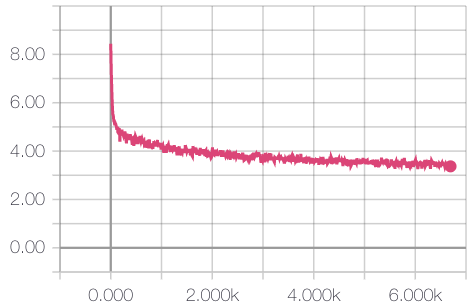
\includegraphics[width=.6\linewidth]{training-loss-curve}
  \caption{Loss}
  \label{training-loss-curve}
\end{subfigure}%
\begin{subfigure}{.5\textwidth}
  \centering
  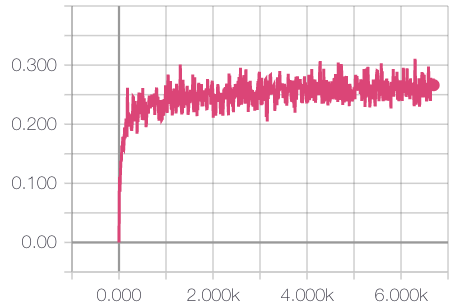
\includegraphics[width=.6\linewidth]{training-recall-curve}
  \caption{Recall@1}
  \label{training-recall-curve}
\end{subfigure}
\caption{Learning curves on the training set. The X-axis is number of steps.}
\label{curves}
\end{figure}

\begin{table}
  \caption{Results for the best model using only merchant name.}
  \label{training-table}
  \centering
  \begin{tabular}{l|ll|l}
    \toprule
    Metric &
    		Training &
    		Validation &
    		Test \\
    \midrule
    	Recall@$1$ & 0.263 & 0.253 & 0.275 \\
    	Recall@$3$ & 0.442 & 0.418 & 0.447 \\
    	Recall@$10$ & 0.644 & 0.602 & 0.614 \\
    	Recall@$1 \mid 5$ & 0.609 & 0.562 & 0.578 \\
    	Loss & 3.46 & 3.04 & 3.25 \\
    \bottomrule
  \end{tabular}
\end{table}

\begin{table}
  \caption{Some of the hyperparameter variations evaluated. Values shown here were computed on the validation set. Lower loss is better.}
  \label{hparams-table}
  \centering
  \begin{tabular}{ll|llll}
    \toprule
    Layer Count &
    		Sequence Length &
    		Recall@$1$ &
    		Recall@$1 \mid 5$ &
    		Loss &
    		Duration (mins)\\
    \midrule
    4 & 32 & \textbf{0.253} & \textbf{0.562} & 3.04 & 42  \\
     & 256 & 0.243 & 0.545 & \textbf{0.501} & \textbf{12} \\
    12 & 32 & 0.252 & 0.561 & 3.04 & 50  \\
     & 256 & 0.234 & 0.536 & 0.529 & 17 \\
    \bottomrule
  \end{tabular}
\end{table}

\begin{table}
  \caption{Some of the feature combinations evaluated. Values shown here were computed on the validation set, by a model with 4 layers given a sequence length of 32, and ran for 20 epochs. Lower loss is better.}
  \label{features-table}
  \centering
  \begin{tabular}{l|lll}
    \toprule
    Feature Combinations &
    		Recall@$1$ &
    		Recall@$1 \mid 5$ &
    		Loss \\
    \midrule
    Merchant name only & 0.253 & 0.562 & 3.04 \\
    Merchant name and MCC & \textbf{0.255} & \textbf{0.563} & \textbf{3.03} \\
    Merchant name, and Time & 0.254 & 0.560 & 3.05 \\
    Merchant name, MCC, and Time & 0.255 & 0.562 & 3.03 \\
    \bottomrule
  \end{tabular}
\end{table}

\subsubsection{Best model}
Table \ref{training-table} summarizes training, validation, and test metrics for the best performing model. This architecture had 4 Transformer layers and used sequences of length 32. It ran for 20 epochs. Figures \ref{training-loss-curve} and \ref{training-recall-curve} show loss and recall curves on the training set for next merchant prediction.  In general, the model did most of its learning in the first 1000 steps of training and then proceeded much more slowly.

Interestingly, validation loss is lower than training loss which is unexpected, despite the evaluation metrics being lower on the validation set, which is expected. This could be explained by less variety in the validation set, since it uses sequences of transactions taken from shorter period of time.

Another fascinating point to call out here is that our test set was taken from a time when consumer behaviour looked much different than it did during the time used for the training set. Training data is all from before January 1st, 2020, and the test set is from April 2020, while the economy was heavily impacted by social distancing. The fact that our model performs just as well on this shifted data distribution could mean one of two things; the predictions it's making are somewhat trivial and  therefore invariant to most behaviour change, or the way consumers changed their behaviour during social distancing was predictable based on how they were behaving previously. This is an open question that my be worth exploring in future work.


\subsubsection{Model Variations}

Table \ref{hparams-table} summarizes a select group of model variations. We were surprised to see that adding more layers did not improve performance. Training on longer sequences was not more accurate but much more more resource-efficient. The discrepancy in loss values between shorter and longer sequences is something that should be investigated. Having much lower loss on longer sequences but not seeing a corresponding increase in the evaluation metrics suggests the loss calculation is taking padded tokens into account and this may be an error.

Table \ref{features-table} summarizes some of the feature combinations evaluated. The complete set combinations was not exhaustively explored but the combinations we did evaluate showed little improvement on the performance of next merchant prediction, despite in most cases decreasing loss on the auxilliary features. The exception to this observation was the amount feature, which the model was not able to learn well and would often cause instability during training.

\subsection{Re-using Representations}

\begin{table}
  \caption{Reference classifier trained on \texttt{gensim} merchant representations.}
  \label{gensim-eval}
  \centering
  \begin{tabular}{l|lll}
    \toprule
    Classification &
    		Precision &
    		Recall &
         F1-score \\
    \midrule
    Partner merchant & 0.70 & 0.04 & 0.07 \\
    Competitor 1 & 0.65 & 0.84 & 0.73 \\
    Competitor 2 & 0.76 & 0.67 & 0.71 \\
    Not relevant & 0.80 & 0.81 & 0.81 \\
    \midrule
    Weighted avg. & 0.73 & 0.72 & 0.70 \\
    \bottomrule
  \end{tabular}
\end{table}

\begin{table}
  \caption{Reference classifier using our model's learned merchant representations.}
  \label{merchant-rep-eval}
  \centering
  \begin{tabular}{l|lll}
    \toprule
    Classification &
    		Precision &
    		Recall &
         F1-score \\
    \midrule
    Partner merchant & 0.83 & 0.02 & 0.04 \\
    Competitor 1 & 0.67 & 0.83 & 0.74 \\
    Competitor 2 & 0.75 & 0.73 & 0.74 \\
    Not relevant & 0.80 & 0.80 & 0.80 \\
    \midrule
    Weighted avg. & 0.74 & 0.73 & 0.70 \\
    \bottomrule
  \end{tabular}
\end{table}

\begin{table}
  \caption{Reference classifier using our model's learned user representations.}
  \label{user-rep-eval}
  \centering
  \begin{tabular}{l|lll}
    \toprule
    Classification &
    		Precision &
    		Recall &
         F1-score \\
    \midrule
    Partner merchant & 0.21 & 0.04 & 0.07 \\
    Competitor 1 & 0.38 & 0.89 & 0.53 \\
    Competitor 2 & 0.52 & 0.22 & 0.31 \\
    Not relevant & 0.66 & 0.19 & 0.29 \\
    \midrule
    Weighted avg. & 0.49 & 0.42 & 0.36 \\
    \bottomrule
  \end{tabular}
\end{table}

Table \ref{gensim-eval} shows the results from the evaluation classifier that uses the baseline \texttt{gensim} merchant representations as input. We note that this method does well overall, but very rarely predicts our partner merchant. This may only be because the data sample used to train this classifier was not balanced with respect to the partner merchant and its competitors, and so our partner merchant accounts for only $<10\%$ of transactions in the sample.

Table \ref{merchant-rep-eval} shows that when the reference classifier is trained using the merchant representations learned by the Transformer model, essentially equal results are achieved. This tells us that our Transformer model has successfully encoded meaningful information about about each merchant in its representations, but fails to beat the baseline.

Table \ref{user-rep-eval} shows that the learned user representations are not as good as simply averaging merchant vectors. This could be because there was not any explicit signal used during training of the Transformer model to propagate information back from the loss function to the user embedding layer. This evaluation may also be suffering because, as mentioned in Section 8.1, our Transformer experiments were performed on a subset of users, which limited the size of the input data for this run of the reference classifier.

\subsection{Projections of Representation Spaces}

\begin{figure}
\centering
\begin{subfigure}{.5\textwidth}
  \centering
  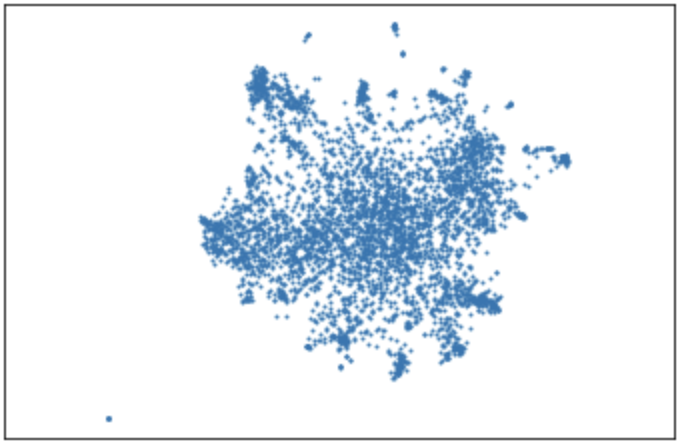
\includegraphics[width=.6\linewidth]{gensim-proj}
  \caption{Baseline}
  \label{gensim-proj}
\end{subfigure}%
\begin{subfigure}{.5\textwidth}
  \centering
  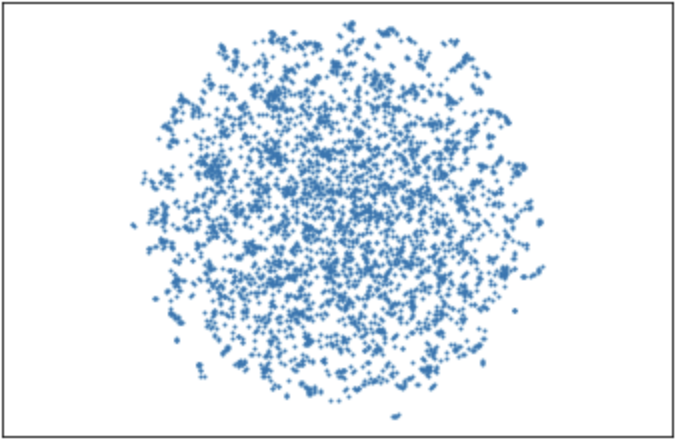
\includegraphics[width=.6\linewidth]{merch-rep-proj}
  \caption{Learned by our model}
  \label{merch-rep-proj}
\end{subfigure}
\caption{Two dimensional projections of merchant representations}
\label{projections}
\end{figure}


In order to begin to form an intuitive understanding of the information actually encoded in merchant representations, we projected them into two dimensions and performed clustering with the hopes of finding semantically meaningful clusters. In this section we compare the projection of our learned merchant representations in Figure \ref{merch-rep-proj} against those obtained with the baseline method in Figure \ref{gensim-proj}. In a manual review we found that the baseline merchant representations displayed more semantically meaningful clusters than our learned representations, however still not as interesting as one would expect when performing the same analysis on a natural language dataset. It is not surprising that our model failed to beat the baseline in this respect since our training did not include any specific task designed to spatially encode semantic information in the representational space. As we can see in Figure \ref{merch-rep-proj}, projected embeddings are more or less normally distributed, whereas Figure \ref{gensim-proj} shows much clearer regions of density. 

\section{Conclusion and future work}
\paragraph{Predictability vs. stochasticity} Given the results shown here we conclude that our model is able to learn useful representations that enable non-trivial prediction of a user's next merchant, and can be used with success as input for other algorithms and other tasks. Achieving a score of $\sim0.25$ on next merchant prediction is not as strong as we were hoping for but is also large enough to show that our model has done meaningful learning. However it seems likely that the processes which generate our observed sequences of transactions are practically stochastic, that is to say, influenced by so many immeasurable factors that they essentially look random. A very interesting direction would be to analyze the algorithmic complexity of merchant sequences according to \cite{Gauvrit:2011}, which relates the randomness of a sequence with the length of the shortest program that can generate that sequence. Recent methods \cite{Zenil:2012} have made this more computationally tractable, however the number of symbols in our case (number of merchants) is still quite likely too large for this analysis to be feasible for now.

\paragraph{Weighted loss} When we sample predictions we notice that the most common merchants are predicted too often in the output, and many merchants are never predicted. This is likely due to an imbalanced distribution of merchants, and in the future this could be addressed by using a weighted loss function, where the value of the weight for each merchant corresponds to the inverse frequency of that merchant in the whole dataset.

\paragraph{Semantic embedding} Much more can be done to improve the downstream utility of the Transformer model's merchant and user representations. We envision adding a training task that helps to spatially encode semantic information about merchants in the embedding space. Such an embedding would ideally be more useful for clustering merchants and users.

\paragraph{Explainability} Being able to explain the predictions of any neural network is an open area of research that may be fruitful to apply to our model. Examining the attention weights could give us valuable insight into relationships between merchants. We also will need to produce some form of explanation if this work is to be used in more regulated domains such as loan adjudication or credit modelling, two active and valuable areas for KOHO. Digging deeper into what the model has learned may also produce valuable insights about consumer behaviour, such as why it's performance did not decrease when performing inference on inputs shifted by the effects of social distancing.

\section{Acknowledgement}
This work has been funded by the NRC-IRAP program and KOHO Financial.

\bibliographystyle{plain}
\bibliography{refs}



\end{document}